\section{hypothesis algorithm}%
\label{sec:halgorithm}
this section starts with a simple example that generates and executes the hypothesis to drive toward a target pose. Then the search and execution loop are discussed, that constitude the principal components of the proposed \ac{halgorithm}. Stepwise, the terminology is elaborated upon whilst an an example of a pushing task is discussed. Then two more examples are provided that involve a blocked path and detecting faults during task execution. Finally, the pseudocode can be resented, supported by a proposed \ac{halgorithm} flowchart.\bs

Two arguments initialize the \ac{halgorithm}, first, a set of object geometry that contains the dimensions of the objects in the robot environment for inernal representation, and second a task to solve.\bs

Additionally several parameters must be specified, such as the grid size, maximum allowed input to the robot and tuning parameters for the path estimator, the path planner and controllers. When all arguements and parameters are provided, the \ac{halgorithm} can be is initialized. There is only a single access point toward the \ac{halgorithm}, the \textit{Respond(observation)} function. This function takes an environment \textit{observation} that updates the internal objects' poses. The function \textit{Respond($\cdot$)} returns control input for the robot. In this thesis, the sensor measurements coinside with the poses objects in the environment. Recall that the perfect-sensor assumption, assumption~\ref{assumption:perfect_object_sensor}, makes access to every object's exact configuration possible.\bs

Now a relatively simple example is presented to indicate how the \ac{halgorithm} operates, later every step will be extensively eleborated. The task in the example consists of driving to a single target pose. The leftmost subfigure in \cref{fig:robot_drive_hgraph} visualizes the initialization of a start and target node, which are connected with a drive action edge in the center figure. To make the drive edge ready for execution in the center subfigure, a system model must be provided to the controller residing in the drive action edge. Motivating the \textit{sys. iden} edge and the \textit{robot\_model} node in the rightmost subfigure.\bs

\begin{figure}[h]
    \centering
    \begin{subfigure}{.3\textwidth}
    \centering
    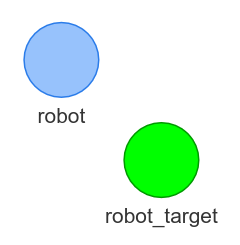
\includegraphics[width=0.7\textwidth]{figures/proposed_method/connecting_nodes/robot_to_target/robot_to_target}
    \end{subfigure}
    \begin{subfigure}{.3\textwidth}
    \centering
    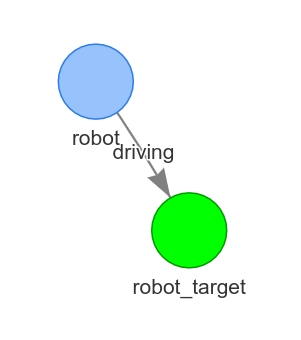
\includegraphics[width=0.9\textwidth]{figures/proposed_method/connecting_nodes/robot_to_target/robot_drive_target}
    \end{subfigure}
    \begin{subfigure}{.3\textwidth}
    \centering
    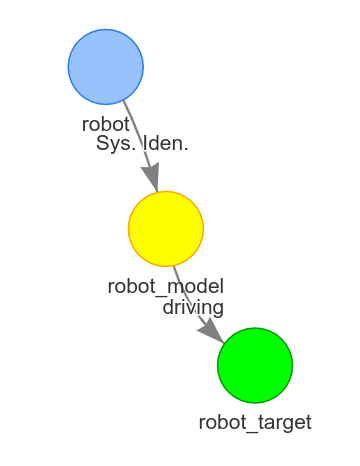
\includegraphics[width=\textwidth]{figures/proposed_method/connecting_nodes/robot_to_target/robot_iden_drive_target}
    \end{subfigure}
    \caption{the \ac{hgraph} in multiple stages when the \ac{halgorithm} searches for an hypothesis to a drive task.}%
    \label{fig:robot_drive_hgraph}
\end{figure}

Now that an hypothesis is created that consists of an identification- and an action edge, the \ac{halgorithm} alternates from the search loop to the execution loop, both loops are addressed shortly. In the execution loop, the \ac{halgorithm} executes the edges by sending input toward the robot, which can be visualized in the figure below.\bs

\begin{figure}[h]
    \centering
    \begin{subfigure}{.3\textwidth}
    \centering
    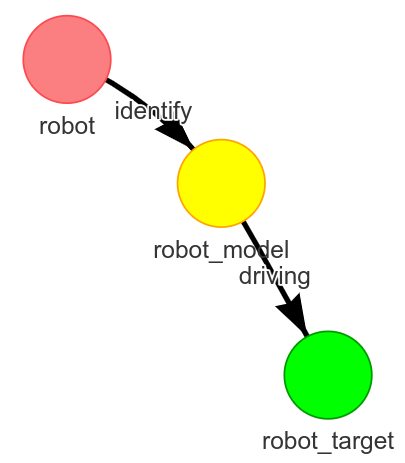
\includegraphics[width=0.9\textwidth]{figures/proposed_method/connecting_nodes/robot_to_target/execute_robot_to_target_1}
    \end{subfigure}
    \begin{subfigure}{.3\textwidth}
    \centering
    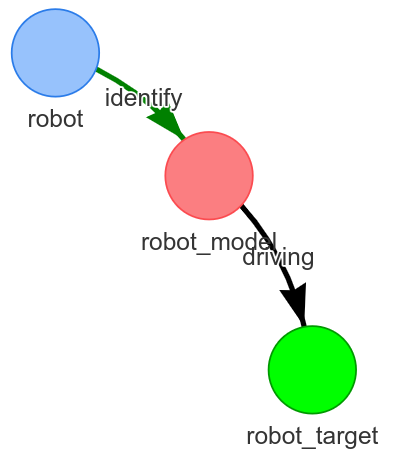
\includegraphics[width=0.9\textwidth]{figures/proposed_method/connecting_nodes/robot_to_target/execute_robot_to_target_2}
    \end{subfigure}
    \begin{subfigure}{.3\textwidth}
    \centering
    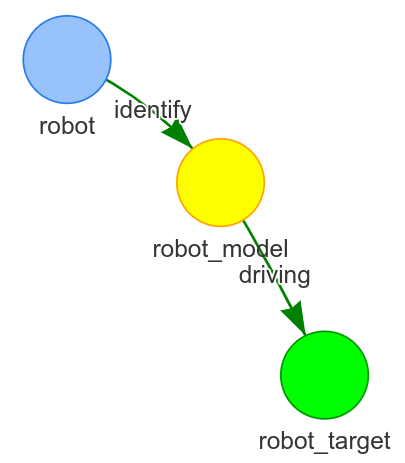
\includegraphics[width=0.9\textwidth]{figures/proposed_method/connecting_nodes/robot_to_target/execute_robot_to_target_3}
    \end{subfigure}
    \caption{executing the hypothesis found in \cref{fig:robot_drive_hgraph}.}
    \label{fig:execute_robot_to_target}
\end{figure}

The generated and executed example for a driving task just discussed is provided to show a simple example. It leaves many details out, which are now elaborated. Start with initializing start- and target nodes, then the search- and execution loop are eleborated.\bs

\paragraph{Initialisation of the \ac{halgorithm}}
the \ac{halgorithm} is initialized with a task that consists of one or more subtasks. Start- and target nodes are created for every subtask, and their status is set to INITIALIZED. Then the goal of the \ac{halgorithm} is to connect every starting node to its corresponding target node with a hypothesis. The target node's status is set to COMPLETED when a hypothesis is completed successfully. If the \ac{halgorithm} could not find a hypothesis that completes a subtask, the \ac{halgorithm} concludes it cannot complete that subtask, and the target node's status is set to FAILED.\bs

\paragraph{The Search and the Execution Loop}
the proposed algorithm comprises two main parts, a search loop and an execution loop. The \ac{halgorithm} searches for a hypothesis in the search loop. In the executions loop, the \ac{halgorithm} tests hypotheses by executing the edges which form the hypothesis. This chapter finaized with a flowchart in \cref{tikz:flowchart_halgorithm} that will be familiar to the following figure where the two main loops can be identified.\bs

\begin{figure}[h]
    \centering
    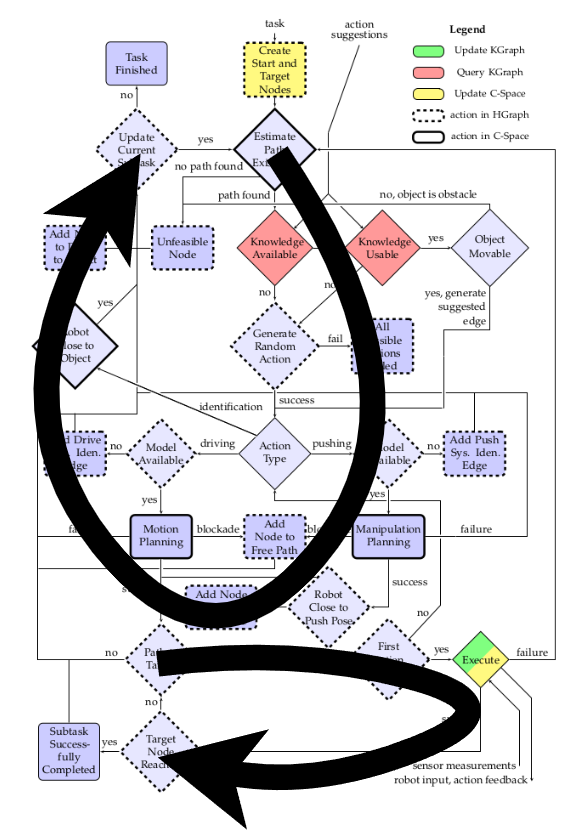
\includegraphics[width=7cm]{figures/proposed_method/two_loops_identified}
    \caption{the search (above) and execution (below) loop, that make up the two main parts of the proposed \ac{halgorithm}. The full flowchart is presented in \cref{tikz:flowchart_halgorithm}}%
    \label{fig:two_loops_identified}
\end{figure}

Hypotheses are formed while the \ac{halgorithm} resides in the search loop. Forming a hypothesis generates nodes, edges, and progressing their status as described in \cref{tikz:status_identification_edge,tikz:status_action_edge}. In the execution loop \textit{an edge is being executed}, a phrase to describe that the controller residing in an edge is sending control input toward the robot. The \ac{halgorithm} operates synchronously. The result is that the robots cannot operate whilst the \ac{halgorithm} resides in the search loop, and during execution, no hypothesis can be formed or updated. The \ac{halgorithm} alternates between the search and execution loop; when in the search loop, a hypothesis is generated, that hypothesis is tested in the execution loop. The execution loop executes the edges that form the hypothesis one by one until either a fault is detected or the hypothesis is completed. Upon fault or completion, the \ac{halgorithm} alternates back to the search loop\bs

When entering or re-entering the search loop, the first thing to determine is if there are unfinished subtasks and, if unfinished subtasks exist, which nodes to connect in order to form a hypothesis that completes that subtask. For such functionality three functions are created; \textit{SubtaskNotFinished}, \textit{GoBackward(\gls{node})}, \textit{FindCorrespondingNode(\gls{node})}. These functions are now discussed.\bs

When elaborating the \ac{halgorithm}, an example presents a visual example with every step in the \ac{halgorithm}. In this example, the robot generates a hypothesis to complete a pushing task that contains a single subtask, initialization and the first generated edges are presented in \cref{fig:robot_push_1}.\bs

\paragraph{finding unfinished subtasks}
determining if there exists an unfinished subtask is validated with the \textit{SubtaskNotFinished(\gls{task})} function. It checks the status for every target node in \ac{hgraph}. The three statuses are; initialized, completed and failed. A target node with an initialized status corresponds to an uncompleted subtask and is returned by the \textit{SubtaskNotFinished(\gls{task})} function. If all existing target nodes have either a completed or failed status, the \ac{halgorithm} concludes that the task is completed.\bs

\paragraph{creating a hypothesis for a subtask}
suppose the \textit{SubtaskNotFinished} returns a target node corresponding to an unfinished subtask. In that case, the \ac{halgorithm} starts searching for a hypothesis connecting the start node to the target node. In \cref{subfig:robot_push_1}, the nodes to connect are the \textit{box} node to the \textit{box\_target} node. These two nodes are a start- and a target node, the nodes to connect are not necessarily start- and target nodes themselves, as seen in \cref{subfig:robot_push_2}. Here the \textit{robot} node must be connected to the \textit{box} node. These nodes are both starting nodes. The first challenge is to find the two nodes to connect from an unfinished target node.\bs

 The \ac{halgorithm} relies on a backward search technique. The backward search technique can be described as \textit{start the search at a goal state and work backwards until the initial state is encountered~\cite{lavalle_planning_2006}.} A motivation for a backward search over a forward search is that it might be the case that the branching factor is significant when starting from the initial state. In such cases, it might be more efficient to use a backward search. If the \textit{SubtaskNotFinished} returns an unfinished subtask, the \ac{halgorithm} starts searching for a hypothesis connecting the start node to the corresponding target node. The first step is to find the right nodes in the \ac{hgraph}, which is now discussed.\bs

 the \textit{GoBackward($\gls{node}_\mathit{target}$)} function takes the a target node $\gls{node}_\mathit{target}$ that corresponds to a unfinised subtask. It then traverses backwards via non-failed edges to find the node that points toward the target node. The function stops traversing back when it encounters a node with a FAILED status or when no edge exists to traverse backwards over. It returns the last node, that node points toward the target node over a sequence of edges with a status other than failed, and all these edges point toward nodes with a status other than failed. In \cref{subfig:robot_push_1} the \textit{GoBackward($\gls{node}_\mathit{box\_target})$} function retuns the $\gls{node}_\mathit{box\_target}$ node, in \cref{subfig:robot_push_2} the \textit{GoBackward($\gls{node}_\mathit{box\_target})$} returns the $\gls{node}_\mathit{box}$ node.\bs

The \textit{GoBackward($\gls{node}_\mathit{target}$)} finds a node to connect to, a corresponding node is sought to connect from, which the \textit{FindCorrespondingNode(\gls{node})} does. \textit{FindCorrespondiNgnode(GoBackward(\gls{node}))} takes a node as parameter and returns an existing node that contains the same object as its arguments node; if such a node does not exist, a new node is created. In both \cref{subfig:robot_push_2,subfig:robot_push_3}, \textit{FindCorrespondingNode(GoBackward($\gls{node}_\mathit{target}$))} returns node $\gls{node}_\mathit{box}$. The nodes that the \ac{halgorithm} desires to connect are renamed to prevent long function names: 
\[\gls{node}_\mathit{to} =  \mathit{gobackward(\gls{node}_\mathit{target})}\]
\[\gls{node}_\mathit{from} = \mathit{findcorrespondingnode(gobackward(\gls{node}_\mathit{target}))}\]

\begin{figure}[h]
    \centering
    \begin{subfigure}{.3\textwidth}
    \centering
    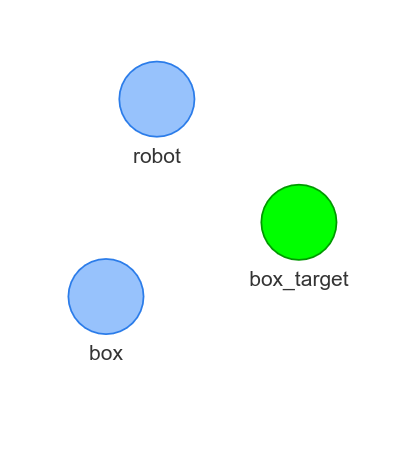
\includegraphics[width=0.8\textwidth]{figures/proposed_method/connecting_nodes/robot_push/robot_push_1}
    \caption{}\label{subfig:robot_push_1}
    \end{subfigure}
    \begin{subfigure}{.3\textwidth}
    \centering
    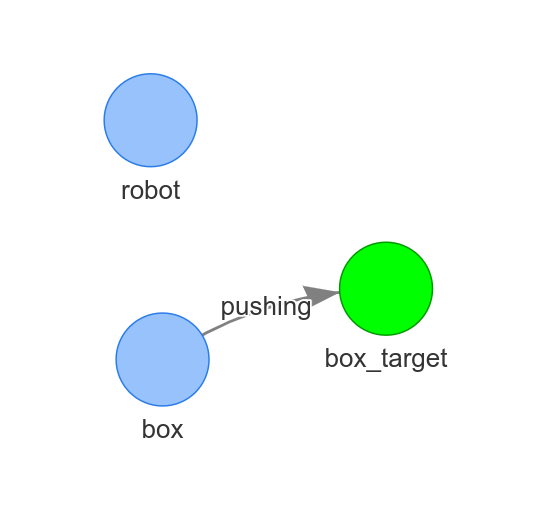
\includegraphics[width=0.8\textwidth]{figures/proposed_method/connecting_nodes/robot_push/robot_push_2_new}
    \caption{}\label{subfig:robot_push_2}
    \end{subfigure}
    \begin{subfigure}{.3\textwidth}
    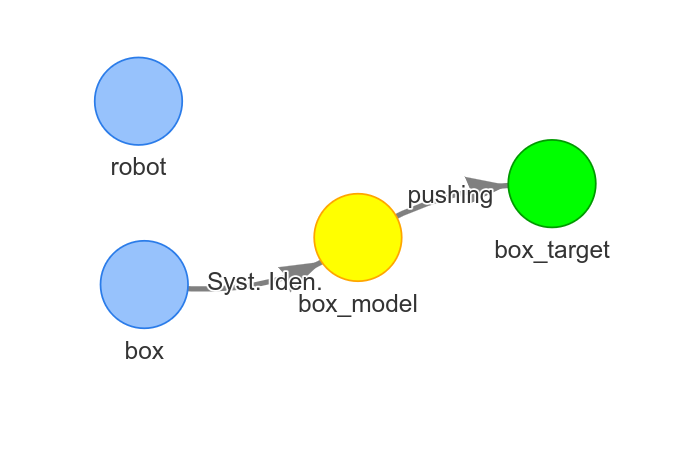
\includegraphics[width=1.1\textwidth]{figures/proposed_method/connecting_nodes/robot_push/robot_push_2}
    \caption{}\label{subfig:robot_push_3}
    \end{subfigure}
    \caption{initialize start and target nodes and the start of a created hypothesis to complete a pushing task.}%
    \label{fig:robot_push_1}
\end{figure}

\paragraph{creating edges}
the \textit{ConnectWithEdge($\gls{node}_1, \gls{node}_2$)} function connects two nodes with an edge, such as the nodes $\gls{node}_\mathit{from}, \gls{node}_\mathit{to}$ just introduced. In this thesis the robot can take two actions, drive and push. It is required that both nodes contain the same object. The push action edge generated and displayed in \cref{subfig:robot_push_2} is between two nodes containing the \textit{box} object. An \textit{EmtpyEdge} is introduced to involve nodes that contain different objects. The emptyEdge serves only to connect nodes that contain different objects and can have status initialized or failed. The \ac{halgorithm} can traverse over emptyEdge if the status is INITIALIZED.\bs


Push action edges require more than only initializing and preparing for execution. The robot must first drive toward a push position against or close to the object to push. By default, creating a push action edge will spawn a $\gls{node}_\mathit{best\_push\_position}$ node connected with an emptyEdge. The \textit{best\_push\_position} depends on the object's planned path. Thus, a path is planned, and then the best push position is determined. \Cref{fig:robot_push_2} shows the $\gls{node}_\mathit{best\_push\_position\_againts\_box}$ node that is connected to the $\gls{node}_\mathit{copy\_box\_target}$. 

\todo{make somehting to teset class of objects}

\paragraph{Valid Hypotheses}
Before a hypothesis can be executed, the hypothesis must be valid. A hypothesis is valid when two conditions are met. First, it starts at the start node and points toward the target node over a sequence of edges with a non-failing status that all point toward nodes with a non-failing status. Second, the first edge in the hypothesis must be ready for execution which the next paragraph will elaborate upon further. To indicate a node or edge has a status other than the FAILED status, that node or edge is called a non-failed node or -edge. To check if an hypothesis is valid the \textit{IsConnected($\gls{node}_1, \gls{node}_2$)} is created. This function checks if there exists a path in the \ac{hgraph} from $\gls{node}_1$ to $\gls{node}_2$ over a sequence of non-failing nodes and -edges. In the pushing task example, the first occurrence of a valid hypothesis is presented in \Cref{subfig:robot_push_4}.\bs

\begin{figure}[H]
    \centering
    \begin{subfigure}{.3\textwidth}
    \centering
    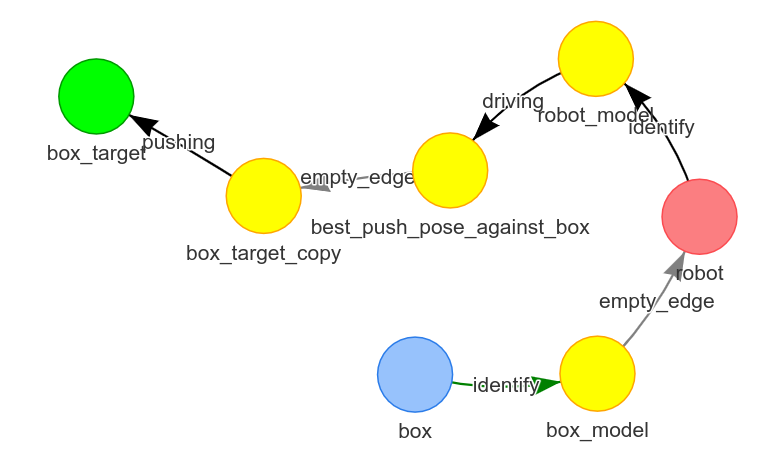
\includegraphics[width=1\textwidth]{figures/proposed_method/connecting_nodes/robot_push/robot_push_4_new}
    \caption{}\label{subfig:robot_push_4}
    \end{subfigure}
    \begin{subfigure}{.3\textwidth}
    \centering
    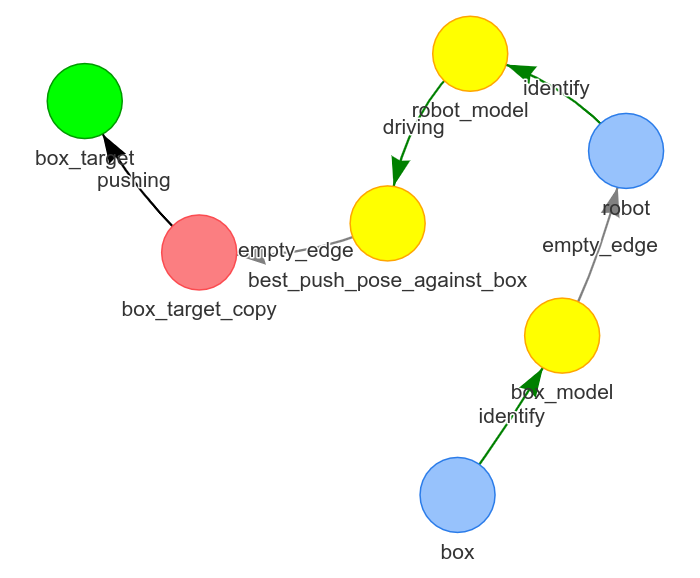
\includegraphics[width=1\textwidth]{figures/proposed_method/connecting_nodes/robot_push/robot_push_5_new}
    \caption{}\label{subfig:robot_push_5}
    \end{subfigure}
    \caption{The hypothesis for a pushing task becomes valid. The hypothesis contains an edge that sends actions to the robot, and thus the hypothesis is executed.}%
    \label{fig:robot_push_2}
\end{figure}

\paragraph{Preparing edges for Execution}
Initialized identification edges are immediately ready to send input toward the robot to collect \ac{IO} data. In contrast to identification edges, action edges must first take several actions in preparation before they are ready to send input toward the robot. The status of an edge indicates at which step of preparing the action edge is, indicated in \Cref{tikz:status_action_edge}. After initialization, the action edge must perform path estimation, load in a system model, perform path planning and then it is ready for execution. Two functions are created to make edges ready for execution. The \textit{ReadyForExecution(\gls{edge})} validates if an edge is ready for execution depending on its status. Identification edges are ready for execution when they bear the INITIALIZED status, and action edges are ready when they bear the PATH PLANNED status. The \textit{MakeReady(\gls{edge})} function takes an edge and takes action depending on its status presented in the following table.\bs

\begin{table}[H]
    \centering
    \begin{tabular}%
    {>{\raggedright\arraybackslash}p{0.25\textwidth}|%
    >{\raggedright\arraybackslash}p{0.65\textwidth}}
      Action edge status& action taken by \textit{MakeReady} function\\\toprule
      INITIALIZED& Create a path estimator and estimate path existence. If no path can be estimated, the status is updated to FAILED. If a path can be estimated, a shortest path is found that acts as a \quotes{warm start} for the path planner.\\
      PATH EXISTS& Load in a system model.\\
      SYSTEM MODEL& Create path planner and plan path. The edge status is updated to FAILED if no path can be found. If a path is found, it acts as a reference signal for the controller. Additionally, the path the planner finds can indicate that an object is blocking. In such cases, the \ac{halgorithm} must first push that object to free the path. An example of such a case is provided in \Cref{fig:blocking_obj_hgraph}.
    \end{tabular}
    \caption{The action edge status is presented in the left column, the corresponding action taken by the \textit{MakeReady} function to prepare an action edge for execution in the right column. An action edge increments its status as indicated in \Cref{tikz:status_action_edge}.}%
    \label{table:make_action_edge_ready}
\end{table}

\paragraph{Hypothesis Execution}
When the \ac{halgorithm} creates a valid hypothesis, it switches from the search loop to the execution loop. Executing a hypothesis is managed by three functions. The first edge in the hypothesis is ready for execution and thus contains a controller and a path to track. That edge is executed, and its controller sends input toward the robot to track the path. The \textit{SteerTowardTarget(\gls{edge})} calculates the input that steers the robot toward the path. The \textit{TargetNotReached(\gls{edge})} validates if the robot has reached the target, which is the last configuration in the path. A margin is set by which the \textit{TargetNotReached(\gls{edge})} concludes that the robot is close enough to the final target pose. For drive actions, that margin is set to 0.1 meters measured in Euclidean instance between the robot and the robot's target position.
For push action, that margin is set to 2 meters, measured in Euclidean distance between the object and the object's target position. These values are tuned by trial and error and is one of the improvements that can be made in future work. The large margin for pushing tasks is set to ensure that the target pose is reached. With a lower margin, the object is often pushed further than the target position. As discussed in the upcoming paragraph, the robot will detect that the object deviated too much from the path. The robot then drives toward the object's opposite side to again, push it over the target position. After the successful completion of an edge, the next edge in the hypothesis is selected by the \textit{IncrementEdge} function. Two possible outcomes exist, the next edge is ready for execution, the \ac{halgorithm} remains in the execute loop, or the next edge is not yet ready. The \ac{halgorithm} goes from the execution loop toward the search loop to prepare the next edge for execution.\bs



\todo{updated figures below}

\begin{figure}[H]
    \centering
    \begin{subfigure}{.3\textwidth}
    \centering
    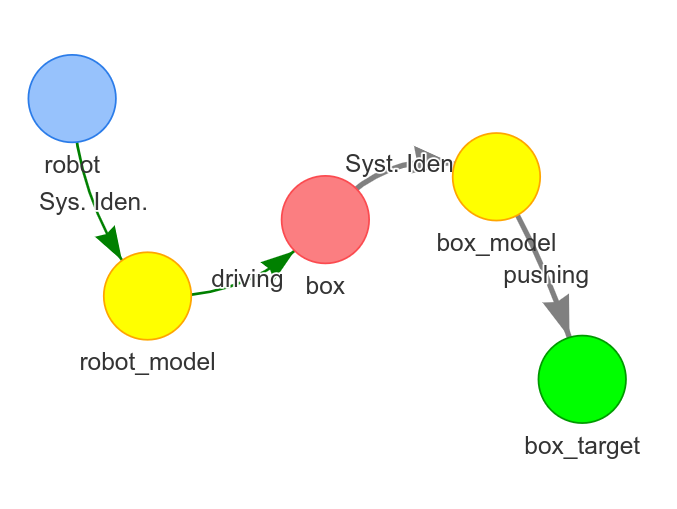
\includegraphics[width=1.05\textwidth]{figures/proposed_method/connecting_nodes/robot_push/robot_push_5}
    \caption{}\label{subfig:robot_push_6}
    \end{subfigure}
    \begin{subfigure}{.3\textwidth}
    \centering
    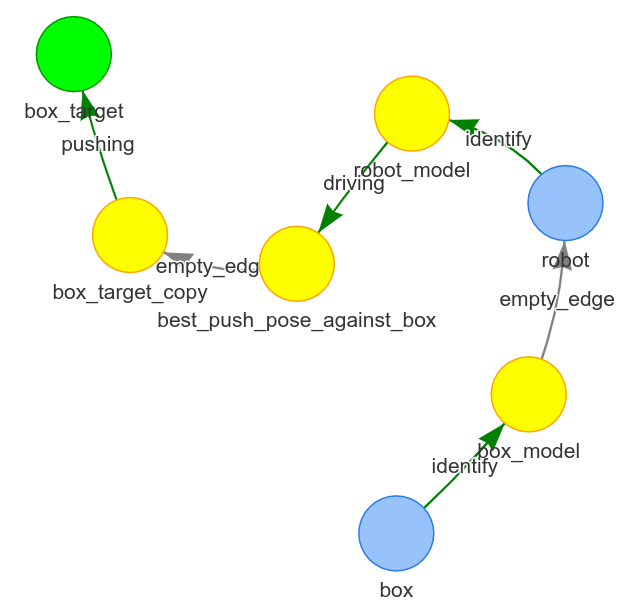
\includegraphics[width=1.05\textwidth]{figures/proposed_method/connecting_nodes/robot_push/robot_push_6}
    \caption{}\label{subfig:robot_push_7}
    \end{subfigure}

    \begin{subfigure}{.3\textwidth}
    \centering
    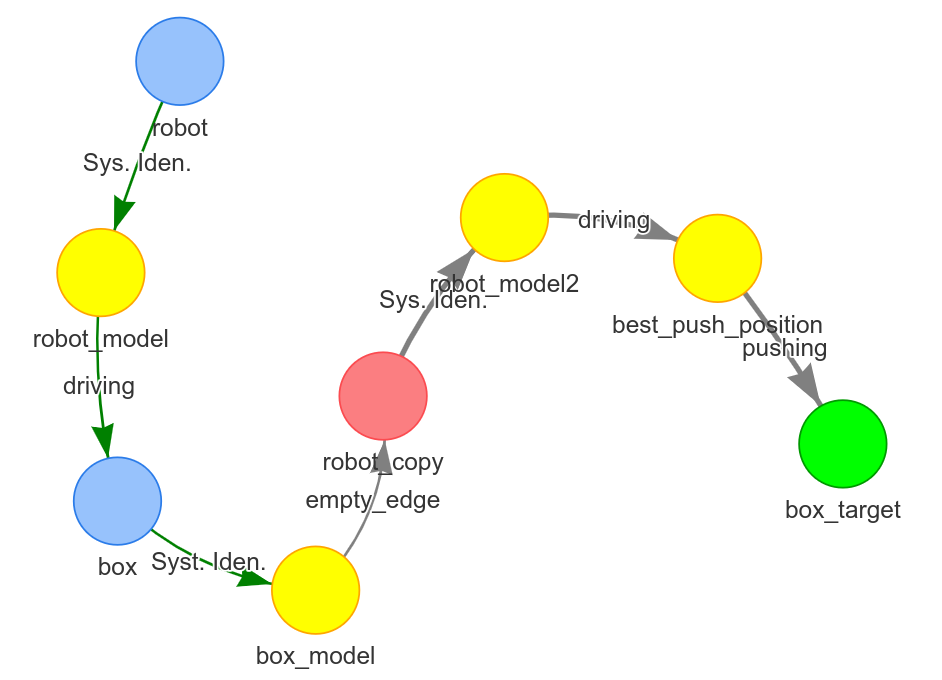
\includegraphics[width=1\textwidth]{figures/proposed_method/connecting_nodes/robot_push/robot_push_7}
    \caption{}\label{subfig:robot_push_8}
    \end{subfigure}
    \begin{subfigure}{.3\textwidth}
    \centering
    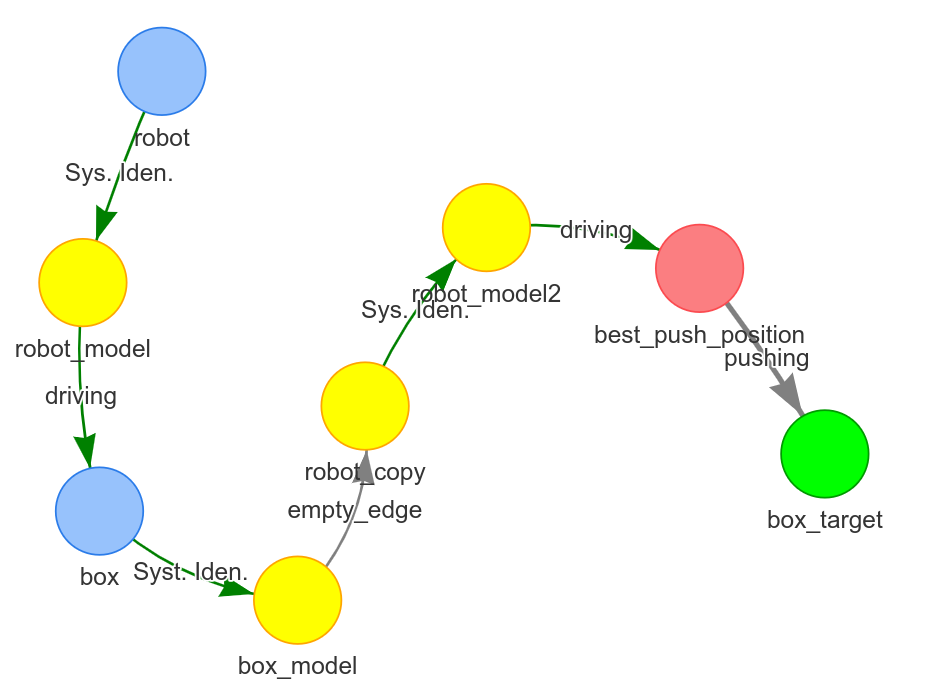
\includegraphics[width=1.05\textwidth]{figures/proposed_method/connecting_nodes/robot_push/robot_push_8}
    \caption{}\label{subfig:robot_push_9}
    \end{subfigure}
    \caption{todo}%
    \label{fig:robot_push_3}
\end{figure}




\paragraph{Successfull Completing Hypotheses and Edges}


\begin{figure}[H]
    \centering
    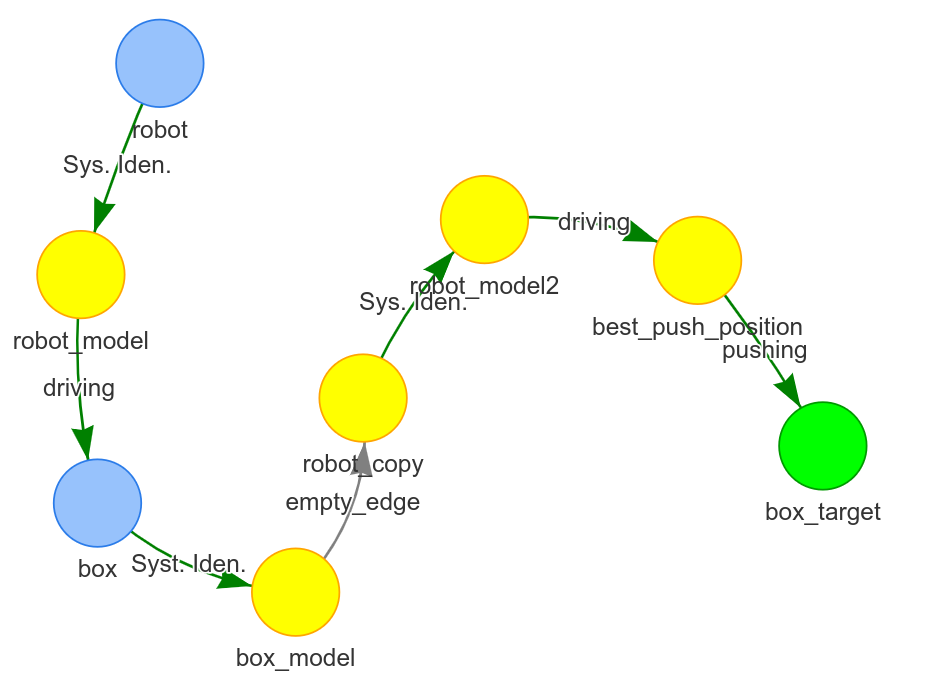
\includegraphics[width=\textwidth]{figures/proposed_method/connecting_nodes/robot_push/robot_push_9}
    \caption{TODO\ac{hgraph} for pushing the green box to the target configuration}%
    \label{fig:robot_push_4}
\end{figure}


\paragraph{Fault Detection}
\todo{This entire section should be merged with the text belwo}

\todo{this below is not a section please c'mon}
\section{Monitoring Metrics}%
\label{sec:monitoring_metrics}
In the next chapter, the proposed framework is discussed, for this section, it is important to know that the proposed framework contains the \ac{halgorithm} which is responsible for finding action sequences, motion/manipulation planning, and execution of drive and push actions. During the execution time of a drive or push action, the \acl{halgorithm} is unable to perform any other action. This blocking behavior has some implications, mainly a controller can steer the system to a state from which it cannot independently reach the target state, as a result, it will never halt. For example, a controller tries to drive the robot toward a target state but there is an unmovable obstacle in the way. Another example is the controller is closed-loop unstable and never reaches its target state. Both examples do not occur is well defined simulation environmnents, because of the \textit{closed-world assumption} defined in \Cref{assumption:closed_world}. In the real world, an unexpected blocking obstacle or unstable controller is more likely to occur.\bs

Detecting controller faults is a large robotic topic~\cite{khalastchi_fault_2019}, properly implementing a fault detection and diagnosis module is out of the scope of this thesis. Instead, two simple metrics will be monitored during execution. The first monitoring metric is \ac{PE}, the second monitoring metric is \ac{TE}. Definitions of the monitoring metrics are summarised in \Cref{table:monitoring_edge_metrics}, it also provides insight in which monitoring metric would catch what faulty behavior. The \ac{PE} and \ac{TE} are defined as:\bs

\[ \gls{pe}(\gls{k}) ::= ||\gls{Cest}(\gls{k}|\gls{k}-1) - \gls{c}(\gls{k})|| \]

Where $\gls{Cest}(\gls{k}|\gls{k}-1)$ is a prediction of the configuration and $\gls{c}(\gls{k})$ is the actual configuration.\bs

The \acl{PE} can be described as:\\
Every time step a prediction one step into the future is made with the use of the system model and system input. Then the system input is applied to the system and the actual configuration is measured. The difference between predicted and actual configuration is defined as:\bs

\[ \gls{te}(\gls{k}) ::= ||\gls{c}_\mathit{target} - \gls{c}(\gls{k})|| \]

Where $\gls{c}_\mathit{target}$ is the target configuration in the path that the controller tries to steer toward, and \gls{c}(\gls{k}) is the actual configuration.\bs

The \acl{TE} can be described as:\\ A path consists of a list of configurations, a controller tracks the path by steering the system to the upcoming configuration in the path when reached the configuration is updated to the next configuration in the path. The difference between the current configuration and the current configuration the controller tries to steer toward is the \ac{TE}.\bs

$\gls{c}_\mathit{target}$ does not update every time step, whilst \gls{c}(\gls{k}) does update every time step. As a result, a \quotes{good} \ac{TE} is expected to take the form of a saw tooth function inverted over the horizontal x-axis.\bs

\noindent
\begin{table}[H]
\centering
\begin{tabular}%
  {>{\raggedleft\arraybackslash}p{0.23\textwidth}%
   >{\raggedright\arraybackslash}p{0.67\textwidth}}
\acf{PE}&  During executing a sudden high \ac{PE} indicates unexpected behavior occurs, such as when the robot has driven into an object which it was not expecting. A high \ac{PE}, which persists indicates that the robot is continuously blocked. Single collisions are allowed, but when the \ac{PE} exceeds a pre-defined threshold and persists over a pre-defined time, the \ac{hgraph} concludes that there was an error during execution and the edge failed.\\
\acf{TE}& The system should not diverge too far from to path it is supposed to track, if the robot diverges more than a pre-defined threshold the \ac{hgraph} concludes that there was an error during execution and the edge fails. \\
\end{tabular}
\caption{Monitor metrics used to monitor if a fault occurred during the execution of an edge}%
\label{table:monitoring_edge_metrics}
\end{table}
During the execution of edges, the progress is monitored every timestep by the \textit{FaultDetected(\gls{edge})} function. A fault is concluded when the \acf{PE} or the \acf{TE} crosses a predefined threshold. The \textit{HandleFault(\gls{edge})} function then updates the executing edge's status to FAILED, and the \ac{halgorithm} switches from the execution loop to the search loop in search for a new hypothesis. The predefined thresholds are split for drive and push actions because driving actions, on average, have much lower \ac{PE} and \ac{TE}. For drive action edges, if the average of the last 25 recorded \ac{PE}'s is higher than 0.05 meter, or the \ac{TE} is higher than 2 meters, a fault is concluded. Only a \ac{TE} is used for push actions, which is split into two parts. One ensures the object follows the path, and another ensures that the robot does not deviate too far from the object. If, for a pushing edge, the object deviates more than 2 meters from the path or the robot deviates more than 2 meters from its push position determined by the object pose, a fault is concluded.\bs

\paragraph{The Blocklist}%
The blocklist prevents the regeneration of failed edges in the \ac{hgraph}. The infinite loop of creating an edge that fails only to be regenerated is prevented. The blocklist keeps a list of edge parameterization with the node identifier; newly generated edges are checked against this blocklist. If they are on the blocklist, initialization of the edge is prevented. The possible parameterizations are filtered when two nodes are connected with an action edge. Thus, any parameterization on the blocklist for a specific node (to which the action edge would point to) cannot be created again for the lifetime of the \ac{hgraph}.\bs

In the following example, \Cref{fig:failure_in_hgraph} faults are detected, these edges are added to the blocklist, the first hypothesis fails to complete, and the \ac{halgorithm} tries to generate a new hypothesis that also fails to complete.\bs

\begin{figure}[H]
    \centering
    \begin{subfigure}{.3\textwidth}
    \centering
    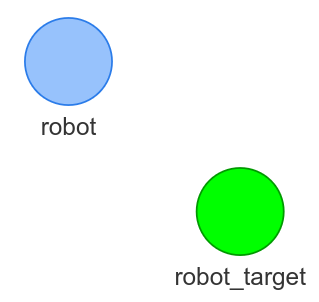
\includegraphics[width=0.8\textwidth]{figures/proposed_method/connecting_nodes/failure/fail_1}
    \end{subfigure}
    \begin{subfigure}{.3\textwidth}
    \centering
    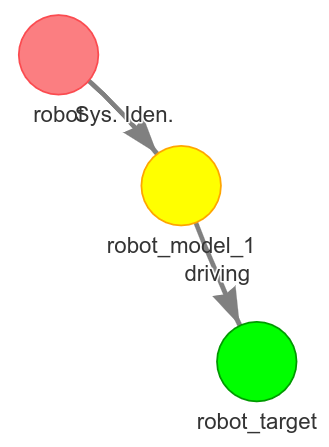
\includegraphics[width=1.05\textwidth]{figures/proposed_method/connecting_nodes/failure/fail_2}
    \end{subfigure}
    \begin{subfigure}{.3\textwidth}
    \centering
    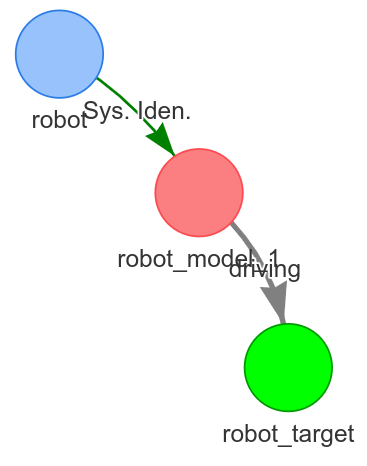
\includegraphics[width=\textwidth]{figures/proposed_method/connecting_nodes/failure/fail_3}
    \end{subfigure}

    \begin{subfigure}{.3\textwidth}
    \centering
    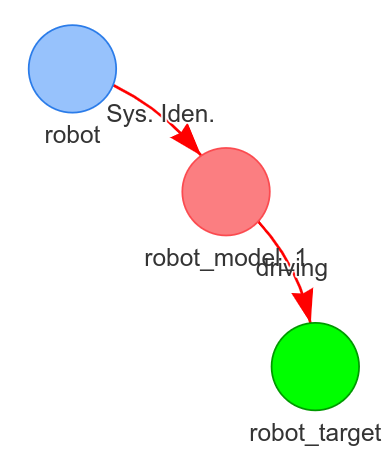
\includegraphics[width=1\textwidth]{figures/proposed_method/connecting_nodes/failure/fail_4}
    \end{subfigure}
    \begin{subfigure}{.3\textwidth}
    \centering
    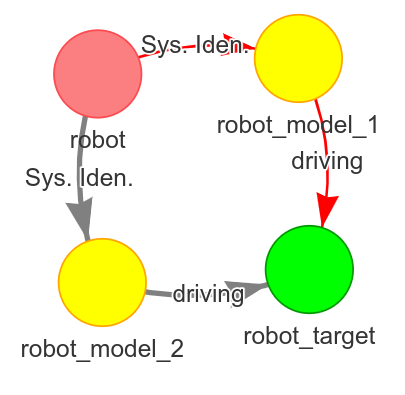
\includegraphics[width=1\textwidth]{figures/proposed_method/connecting_nodes/failure/fail_5}
    \end{subfigure}
    \begin{subfigure}{.3\textwidth}
    \centering
    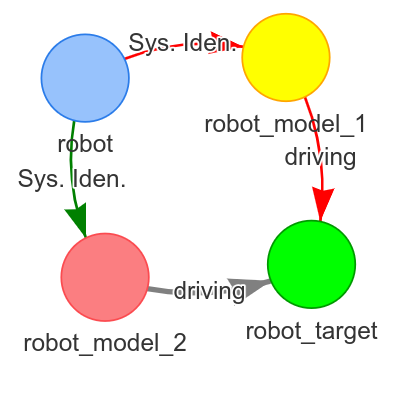
\includegraphics[width=1\textwidth]{figures/proposed_method/connecting_nodes/failure/fail_6}
    \end{subfigure}

    \begin{subfigure}{.3\textwidth}
    \centering
    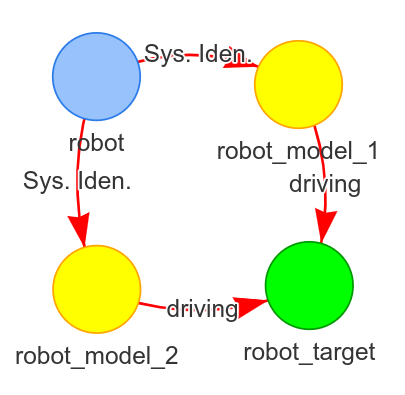
\includegraphics[width=1\textwidth]{figures/proposed_method/connecting_nodes/failure/fail_7}
    \end{subfigure}
    \hfill
    \caption{Executing two hypotheses that both failed to complete because a fault was detected. Both edges are added to the blocklist, preventing the regeneration of edges with the same parameterization. The \ac{halgorithm} concludes the task to be unfeasible.}%
    \label{fig:failure_in_hgraph}
\end{figure}

In \Cref{fig:failure_in_hgraph}, only two parameterizations of drive controllers and system models were available. Thus after two failed hypotheses, the \ac{halgorithm} concludes that the task is unfeasible. All functionality is now discussed and is neatly summarized in the following table. Then, pseudocode for the proposed \ac{halgorithm} is presented.\bs

\begin{table}[H]
\centering
\begin{tabular}%
  {>{\raggedright\arraybackslash}p{0.25\textwidth}%
   >{\raggedright\arraybackslash}p{0.65\textwidth}}
\textit{SubTaskNotFinished(\gls{subtask})}:& Return False if the subtask \gls{subtask} is completed or it is concluded to be unfeasible \\
\textit{IsConnected($\gls{node}_1, \gls{node}_2$)}:& Return True if there exist a path in the \ac{hgraph} from node $\gls{node}_1$  to node $\gls{node}_2$ through a number of non-failed edges\\
\textit{ReadyForExecution(\gls{edge})}: & Return True if the edge \gls{edge} is ready to execute\\
\textit{TargetNotReached(\gls{edge})}: & Return True edge \gls{edge} has not reached it target configuration\\
\textit{FaultDetected(\gls{edge})}: & Return True if a fault has been detected during execution of edge \gls{edge}\\

\textit{HandleFault(\gls{edge})}: & Update edge \gls{edge} status to FAILED and remove edge from hypothesis \\
\textit{SteerTowardTarget(\gls{observation})}: & Update controller with observation \gls{observation} and compute response that steers the system to target configuration\\
\textit{ReadyForExecution(\gls{edge})}: & Check if edge \gls{edge} has the PATH PLANNED status and contains all components to control the system \\
\textit{IncrementEdge}: & Mark current edge as completed, set next edge in \gls{hypothesis} as current edge \\
\textit{MakeReady(\gls{edge})}: & Perform actions to make the edge \gls{edge} ready for execution \\
\textit{goBackward(\gls{node})}: & Find the source node that point toward \gls{node} through a number of non-failed edges\\
\textit{FindCorrespondingNode(\gls{node})}: & Find the node containing the same object as \gls{node} \\
\textit{ConnectWithEdge($\gls{edge}_1, \gls{edge}_2$)}: & Randomly generate edge between nodes $\gls{node}_1$ and $\gls{node}_2$ or use \ac{kgraph} to suggest an edge\\
\end{tabular}
\caption{The functions employed by the \ac{halgorithm} in \Cref{pseudocode:halgorithm}.}
\label{table:functions_for_halgorithm}
\end{table}
\todo{Currentedge is nto defined}

\noindent
\begin{algorithm}[H]
  \caption{Pseudocode for the proposed hypothesis algorithm.}\label{pseudocode:halgorithm}
  \begin{algorithmic}[1]

    \hspace{-0.9cm}\colorbox{my_grey}{\parbox{\linewidth}{%
        \For{$\gls{subtask} \in \gls{task}$}

        \hspace{-0.1cm}\colorbox{my_yellow}{\parbox{\linewidth}{%
            \While{\textit{SubTaskNotFinished(\gls{subtask})}}\algorithmiccomment{Search Loop}
            \If{\textit{\gls{hgraph}.IsConnected(\gls{subtask}.start, \gls{subtask}.target)}}
            \If{\textit{\gls{hypothesis}.CurrentEdge.ReadyForExecution}}

            \hspace{-0.1cm}\colorbox{my_light_blue}{\parbox{\linewidth}{%
                \While{\textit{TargetNotReached(\gls{hypothesis}.CurrentEdge)}} \algorithmiccomment{Execution Loop}
                \If{\textit{FaultDetected(\gls{hypothesis}.CurrentEdge)}}
                \State \textit{HandleFault(\gls{hypothesis}.CurrentEdge)}
                \State break
                \EndIf
                \State \textit{\gls{hypothesis}.CurrentEdge.SteerTowardTarget(\gls{observation})}
                \If{\textit{TargetReached(\gls{hypothesis}.CurrentEdge)}}
                \If{\textit{ReadyForExecution(\gls{hypothesis}.CurrentEdge)}}
                  \State \textit{\gls{hypothesis}.IncrementEdge}
                \Else
                  \State break
                \EndIf
                \EndIf
                \EndWhile
            }}
            \Else
            \State \textit{MakeReady(\gls{hypothesis}.CurrentEdge)}
            \EndIf
            \Else
            \State $\mathit{\gls{node}_{localtarget}} \leftarrow \gls{hgraph}.\mathit{goBackward(\gls{node}.target)}$
            \State $\mathit{\gls{node}_{localstart}} \leftarrow \gls{hgraph}.\mathit{findCorrespondingNode(\gls{node}_{localtarget})}$
            \State $\mathit{G.connectWithEdge}(\gls{node}_\mathit{localstart}, \gls{node}_\mathit{localtarget})$
            \EndIf
            \EndWhile
        }}
        \EndFor
    }}
  \end{algorithmic}
\end{algorithm}

A flowchart of the \ac{halgorithm} is presented in \Cref{tikz:flowchart_halgorithm}. Compared to the pseudocode presented above, the flowchart provides more detail, especially in the elaborate description accompanying the flowchart in \Cref{table:explainer_hgraph_figures_nodes}. The flowchart includes a connection point to the \ac{kgraph} and robot environment. The blocks in the flowchart indicate the resources used and changes indicated in the legend. Compared to the flowchart, the pseudocode is an abstract version, leaving many details explicitly related to the robot used in this thesis. Pseudocode encompasses a broader field of robots. So can the pseudocode also be applied to a robot with manipulation abilities other than nonprehensile pushing.\bs

\newpage
\vspace*{-1.2cm}
\hspace{-1.2cm}
\begin{minipage}{10cm}
\begin{figure}[H] 
\centering
\begin{tikzpicture}]
  [node distance = 3cm] 

    % Nodes
    \node [block, fill=yellow!50, line width=2pt, dashed] (first) {Create Start and Target Nodes};
    
    % legend
    \node[text width=2.8cm, yshift=0.6cm, right of=first, node distance=7cm, text centered, rounded corners, minimum height=1em, label={[name=lab, yshift=0.4cm, left]\textbf{Legend}}] (legend1) {\small Update KGraph};
    \node[rectangle, draw, left of=legend1, fill=green!50, rounded corners, minimum height=1em, minimum width=1cm, node distance=2cm] (legend1color) {};
    
    \node[text width=2.8cm, below of=legend1, text centered, minimum height=1em, node distance=0.7cm] (legend2) {\small Query KGraph};
    \node[rectangle, draw, left of=legend2, fill=red!40, rounded corners, minimum height=1em, minimum width=1cm, node distance=2cm] (legend2color) {};
   
    \node[text width=2.8cm, below of=legend2, text centered, minimum height=1em, node distance=0.7cm] (legend3) {\small Update C-Space};
\node[rectangle, draw, left of=legend3, fill=yellow!50, rounded corners, minimum height=1em, minimum width=1cm, node distance=2cm] (legend3color) {};
    
    \node[text width=2.8cm, below of=legend3, text centered, minimum height=1em, node distance=0.7cm] (legend4) {\small action in HGraph};
    \node[rectangle, draw, left of=legend4, rounded corners, minimum height=1em, minimum width=1cm, node distance=2cm, line width=2pt, dashed] (legend4color) {};
 
    \node[text width=2.8cm, below of=legend4, text centered, minimum height=1em, node distance=0.7cm] (legend5) {\small action in C-Space};
\node[rectangle, draw, left of=legend5, rounded corners, minimum height=1em, minimum width=1cm, node distance=2cm, line width=2pt] (legend5color) {};

    % nodes, Path exists 
    \node [decision, below of=first, node distance=2.6cm, line width=2pt] (path_existence) {Estimate Path Existence};
    \node [decision, left of=path_existence, node distance=4.5cm, line width=2pt, dashed] (subtasks) {Update Current Subtask};

    \node [block, above of=subtasks, node distance=2.8cm] (no_solution_found) {Task Finished};
    
    % nodes, Knowledge available
    \node [decision, fill=red!40, below of=path_existence, node distance=3.2cm, inner sep=0.5mm] (know_avail) { Knowledge Available };
    \node [decision, fill=red!40, right of=know_avail, node distance=3.5cm, inner sep=0.5mm] (know_good) {Knowledge Usable};
    \node [decision, right of=know_good, node distance=3.5cm, text width=1.7cm] (movable) {\vspace{0.1cm}\shortstack[]{Object\\Movable}};
    \node [block, left of=know_avail, node distance=3cm, line width=2pt, dashed] (impossible) {Unfeasible Node};
    
    % nodes, Generate new edge
    \node [decision, below of=know_avail, node distance=3.2cm, line width=2pt, inner sep=0.5mm, dashed] (goto_sys_iden) {Generate Random Action};

    \node[block, right of=goto_sys_iden, node distance=3.5cm, line width=2pt, dashed] (no_trans_found) {All Possible Actions Failed};
    
    
    % Motion/Manipulation planning 
    \node [decision, below of=goto_sys_iden, node distance=3.5cm] (single_multi) {Action Type};

    \node [decision, line width=2pt, dashed, left of=single_multi, node distance=3.7cm] (model_avail_single) {Model Available};
    \node [decision, line width=2pt, dashed, right of=single_multi, node distance=3.7cm] (model_avail_multi) {Model Available};
    \node [block, line width=2pt, dashed, left of=model_avail_single, node distance=2.8cm] (sys_iden_single) {Add Drive Sys. Iden. Edge};
    \node [block, line width=2pt, dashed, right of=model_avail_multi, node distance=2.8cm] (sys_iden_multi) {Add Push Sys. Iden. Edge};
    \node [block, line width=2pt, dashed, below of=single_multi, node distance=2.7cm] (move_object) {Add Node to Free Path};
    \node [block, line width=2pt, left of=move_object, node distance=3.7cm] (motion_planning) {Motion Planning};
    \node [block, line width=2pt, right of=move_object, node distance=3.7cm, text width=2.1cm] (manipulation_planning) {Manipulation Planning};

    \node [decision, line width=2pt, dashed, minimum width=2.3cm, below of=move_object, node distance=2.3cm, xshift=1.75cm] (drive_to_push_position) {Robot Close to Push Pose};
    \node [block, line width=2pt, dashed, minimum width=2.3cm, below of=move_object, node distance=2.3cm, xshift=-1.75cm] (goto_push_position) {Add Node to Drive to Push Pose};
  
    \node [decision, line width=2pt, above of=sys_iden_single, node distance=3.5cm] (add_drive_node) {Robot Close to Object};

    \node [block, dashed, line width=2pt, above of=add_drive_node, node distance=3.2cm] (do_add_drive_node) {Add Node to Drive to Object};

    % nodes, Path to target
    \node [decision, below of=motion_planning, node distance=4.0cm, line width=2pt, dashed] (global_path) {Path to Target}; 
1   \node [decision, right of=global_path, node distance=7.4cm, line width=2pt, dashed] (first_action) {First Action Planned};

    \node [decision, right of=first_action, diagonal fill={yellow!50}{green!50}, node distance=3cm] (execute) {Execute};
     
    % nodes, Target node reached 
    \node [decision, below of=global_path, node distance=3cm, line width=2pt, dashed] (target_node_reached) {Target Node Reached};
    \node [block, left of=target_node_reached, node distance=3cm] (end) {Subtask Successfully Completed};
    
    % Edges
    \path[line] ++(0,1.2) -- node[yshift=0.2cm, above]{task} (first);
    \path[line] (first) -- node[midway](to_path_exists){}(path_existence); 
    
    % edges, Path exists 
    \path[line] ([xshift=0.2cm, yshift=-0.2cm] path_existence.south west) -| node[near start, xshift=-0.4cm, above] {no path found} (impossible.north);
    \path[line] (subtasks.north) --  node[left] {no} (no_solution_found);
    \path[line] (path_existence) -- node[xshift=0cm, yshift=0.15cm, left] {path found} (know_avail); 
    \path[line] (subtasks.east) -- node[above] {yes} (path_existence.west);
    
    % edges, Knowledge available
    \path[line] (know_avail) -- node[above] {yes} (know_good); 
    \path[line] (know_good) -- node[yshift=0.1cm, above] {no} (goto_sys_iden); 
    \path[line] (know_avail) -- node[left](toward_new_trans) {no} (goto_sys_iden); 
    \draw[-stealth] (know_good.east) -- node[above] {yes} (movable.west);
    
    % \draw[-]  ([xshift=3.2mm]toward_new_trans.center) -| node[near start, above] {no} (know_good.south);
    \draw[-](impossible.west) -- +(-0.47,0); 
     
    \draw[-]  ([xshift=2.75cm, yshift=6.6cm]know_avail.center) --  node[at start, above] {\shortstack[]{action\\suggestions}} ([xshift=1.75cm, yshift=3.75cm]know_avail.center) -- ([xshift=1.75cm, yshift=3.75cm]know_avail.center);

    \draw[-stealth]  ([xshift=1.75cm, yshift=3.75cm]know_avail.center) --  ([xshift=1.75cm, yshift=1.75cm]know_avail.center) -- (know_avail.north east);
    \draw[-stealth]  ([xshift=1.75cm, yshift=1.75cm]know_avail.center) -- (know_good.north west);
    \draw [draw=white,double distance=\pgflinewidth,ultra thick] (path_existence.east) -- +(2cm,0);
    
    % edges, Generate new edge
    \draw[-] (move_object.south) |- +(-7.70,-0.3);
    \draw [draw=white,double=black,double distance=\pgflinewidth,ultra thick] (motion_planning.south) -- +(0,-1cm);
    \draw[-stealth] (motion_planning.south)  -- ([yshift=-1cm]motion_planning.south) -| node[near start, left] {success} (global_path.north);
    \draw[-stealth] (manipulation_planning.south) |- node[near start, right] {success} (drive_to_push_position.east);
    \draw[-] ([xshift=0.3cm,yshift=0.3cm] drive_to_push_position.north west) -- node[at start, xshift=-0.5cm, above] {yes} ++(-5.05cm,0);
    \draw[-stealth] (drive_to_push_position.west) |- node[xshift=-0.3cm, above] {no} (goto_push_position.east);
    \draw[-] (goto_push_position.west) -- ++(-0.77cm, 0); 

    \draw[-] (motion_planning.west) -- node[above] {failure} +(-2.98,0);
    \draw[-] (manipulation_planning.east) -| node[near start, above] {failure} ([xshift=4.7cm,yshift=-0.6cm]no_trans_found.south) -- ([yshift=-0.6cm]no_trans_found.south);
    
    % edges, Single/Multi body
    \draw[-stealth] (single_multi.west) -- node[above] {driving} (model_avail_single);
    \draw[-stealth] (single_multi.east) -- node[above] {pushing} (model_avail_multi);
    \draw[-stealth] (model_avail_single.south) -- node[left] {yes} (motion_planning.north);
    \draw[-stealth] (model_avail_single.west) -- node[above] {no} (sys_iden_single);

    \draw[-stealth] (model_avail_multi.east) -- node[above] {no} (sys_iden_multi);
    \draw[-stealth] (motion_planning.east) -- node[above] {blockade} (move_object);
    \draw[-stealth] (manipulation_planning.west) -- node[above] {blockade} (move_object);
    \draw[-stealth] (goto_sys_iden) -- node[above] {fail} (no_trans_found);
    \draw[-] (sys_iden_single.north) --  ([yshift=0.56cm]sys_iden_single.north);
    \draw[-] (sys_iden_multi.north) |-  ([yshift=-0.6cm]no_trans_found.south);
    \draw[-] (no_trans_found.south) -- ++(0,-0.6cm) --([xshift=-8cm, yshift=-0.6cm]no_trans_found.south);
    \draw [draw=white,double=black,double distance=\pgflinewidth,ultra thick] (goto_sys_iden.south) -- node[yshift=0.1cm, right] {success}(single_multi.north);
    \draw[-stealth] ([yshift=0.05cm] goto_sys_iden.south) -- (single_multi.north);
    
    \draw[-] (movable.south) |- node[near start, left] {\shortstack[r]{yes, generate\\suggested\\edge}} ([xshift=-1.5cm, yshift=-1.4cm]movable.south) |- ([yshift=0.3cm]single_multi.north);
    \draw [draw=white,double distance=\pgflinewidth,ultra thick]  ([xshift=-1cm]movable.north) |- ([xshift=-7.2cm, yshift=0.15cm]movable.north);

    \draw[-] (movable.north) |- node[xshift=-2cm, above]{no, object is obstacle}([xshift=-10cm, yshift=0.15cm]movable.north);
    % HERE
    \draw [draw=white,double=black,double distance=\pgflinewidth,ultra thick] ([xshift=5.5cm,yshift=0.3cm]single_multi.north) -- ([xshift=5.5cm, yshift=2cm]single_multi.north);
    % \draw[-] (know_good.east) -| node[above]{yes} ([xshift=5.5cm, yshift=0.2cm]single_multi.north) -- ([yshift=0.2cm]single_multi.north);

    
    \draw[-stealth] (add_drive_node.north) -- node[left] {no} (do_add_drive_node.south);
    \draw[-] (add_drive_node.north east) -- node[left] {yes} ++(1.3cm,1.3cm);
    \draw[-] (do_add_drive_node.east) --  ++(1.10cm,0);
    % edges, Path to target
    \path[line] (global_path) -- node[above] {yes} (first_action);
    \path[line] (first_action.east) -- node[above] {yes} (execute);
    \path[line] (global_path.west) -| node[xshift=1cm, left, above, near start] {no}  ([xshift=-2.8cm, yshift=8cm]global_path.west) -|  (subtasks.south); 
   
    \draw[-stealth] (first_action.north east) -- node[near end, left] {no} ([xshift=1.7cm, yshift=0.39cm]first_action.north) |- ([yshift=-0.35cm]single_multi.south) -- (single_multi.south);
    \draw [draw=white,double=black,double distance=\pgflinewidth,ultra thick] (manipulation_planning.east) -- +(1cm,0);
    \draw [draw=white,double=black,double distance=\pgflinewidth,ultra thick] (manipulation_planning.north) -- +(0,0.6cm);
    \draw [draw=white,double=black,double distance=\pgflinewidth,ultra thick] (single_multi.north west) -- ([xshift=1cm,yshift=-0.425cm] add_drive_node.south east);
    \draw[-stealth] (single_multi.north west) -- node[xshift=-0.7cm, yshift=0.4cm, near start, above, right] {identification} (add_drive_node.south east);

    \draw[-stealth] (model_avail_multi.south) -- node[near start, left] {yes} (manipulation_planning.north);
    
    \draw[-stealth] ([yshift=0.2cm, xshift=0.2cm]execute.south east) --  ([yshift=-0.8cm, xshift=1.2cm]execute.south east) -- node[at end, left] {robot input, action feedback} +(0,-2.7cm);
    
    \draw[stealth-] ([yshift=-0.2cm, xshift=-0.2cm]execute.south east) --  ([yshift=-1.2cm, xshift=0.8cm]execute.south east) -- node[left, at end] {sensor measurements} +(0, -1.8cm);
    
    \path[line] (execute.south) |- node[near start, left] {success} (target_node_reached.east);
    \draw[-stealth] (execute.east) -- node[above] {failure} ([xshift=1.5cm]execute.east) |- (path_existence.east);
    \draw[-] (end.north) -- ++(0,2.07cm);
    
    
    % edges, Target node reached 
    \path[line] (target_node_reached.north) -- node[left] {no} (global_path.south);
    \path[line] (target_node_reached.west) -- node[above] {yes} (end.east);

\end{tikzpicture}
% \vspace{-5cm}
\caption{Flowchart displaying the \ac{halgorithm} workflow.}%
\label{tikz:flowchart_halgorithm}% 
\end{figure}

\end{minipage}
\newpage
\todo{I do not think the legend is up-to-date any more}


\begin{table}[H]
\centering
\rowcolors{2}{white}{myLightColor}
\begin{tabular}%
  {>{\raggedright\arraybackslash}p{0.3\textwidth}%
    >{\raggedright\arraybackslash}p{0.7\textwidth}}
\textbf{Node name} & \textbf{Description of actions taken}\\\toprule
Task Finished & log all metrics for the \ac{hgraph}, then deconstruct \ac{hgraph}.\\
Create Start and\newline Target Nodes & Generate a robot node and the start and target nodes for every subtask in the task.\\
Update Current Subtask & Select an unfinished subtask or update the current subtask. Use the backward search technique. The \textit{current\_start\_node} and \textit{current\_target\_node} are updated. When all subtasks have been addressed, conclude task is finished. \\
Estimate Path\newline Existence & Check if a path exists between \textit{current\_start\_node} and \textit{current\_target\_node} whilst assuming that the object is holonomic.\\
Add Node to\newline Drive to Object & Add a node before the \textit{current\_target\_node}.\\
Unfeasible Node & Update node's status to unfeasible because it can not be completed, log failed Edge.\\
Knowledge Available& Query the \ac{kgraph} for action suggestion to connect \textit{current\_target\_node} to \textit{current\_target\_node}\\
Knowledge Usable& Check if a suggested action is not on the blocklist.\\
Object Movable & Check if the object is classified as movable\\
Robot Close to Object& Check if the object is inside directly reachable free space of the robot \\
Generate Random\newline Action& Randomly sample a controller with a compatible system identification method not on the blocklist. \\
All Possible Actions Failed & Every possible action is on the blocklist for the \textit{current\_target\_node}, update \textit{current\_target\_node} status to failed.\\
Add Drive System Identification Edge & Adds an identification edge between a newly generated node and the drive action edge's source node. \\
Model Available& Checks if the drive action edge contains a system model. \\
Action Type& Checks the action type. \\
Model Available& Check if the push action edge contains a system model. \\
Add Push System\newline Identification Edge& Adds identification edge compatible with push action edge. \\
Motion Planning& Search a path for the \textit{current\_edge}, detect blocking objects. \\
Add Node to Free Path & Search close by pose for an object to free the path. Create a node to push the object toward that pose. \\
Manipulation Planning & Search a path for the \textit{current\_edge}, detect blocking objects.\\
Add Node to Drive\newline to Push Pose& Create node to drive toward push pose, add before action edge. \\
Robot Close to\newline Push Pose & Check if the robot overlaps the best push position. \\
Path to Target& Is there a path from robot to target node in the \ac{hgraph}, then set the first edge to \textit{current\_edge} otherwise update subtask.\\
First Action Planned&  Check if motion/manipulation planning was performed. \\
Execute& Execute the \textit{current\_edge}, update \ac{hgraph} after completion, log failed hypothesis if a fault is detected. \\
Subtask Successfully\newline Completed& Log hypothesis metrics. \\
Target Node Reached& Check if the target node is reached.\\
\end{tabular}
\caption{Comprehensive description regarding the actions executed by the blocks in \Cref{tikz:flowchart_halgorithm}.}%
\label{table:explainer_hgraph_figures_nodes}
\end{table}

\paragraph{Encountering a Blocked Path}%
During propagation of an action edge's status, motion or manipulation planning occurs. If an object blocks the path, planning will detect it, and the \ac{halgorithm} tries to free it. In the following example, the \ac{halgorithm} detects a blocking object and frees the path by pushing the blocking object to a new configuration, and can be visualized in \Cref{fig:blocking_obj_hgraph}.\bs

\begin{figure}[H]
    \centering
    \begin{subfigure}{.3\textwidth}
    \centering
    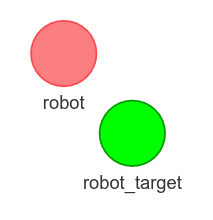
\includegraphics[width=0.6\textwidth]{figures/proposed_method/connecting_nodes/blocking_obj/blocking_obj_1}
    \caption{}
    \end{subfigure}
    \begin{subfigure}{.3\textwidth}
    \centering
    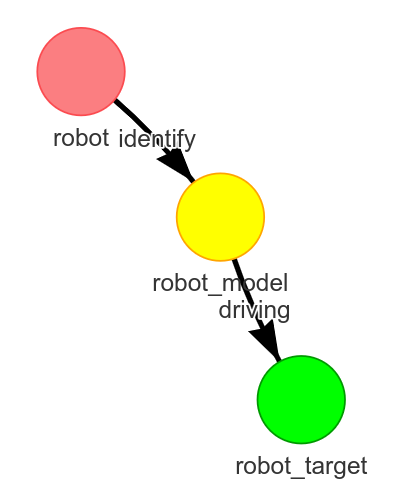
\includegraphics[width=0.9\textwidth]{figures/proposed_method/connecting_nodes/blocking_obj/blocking_obj_2}
    \caption{}\label{subfig:blocking_obj_2}
    \end{subfigure}
    \begin{subfigure}{.3\textwidth}
    \centering
    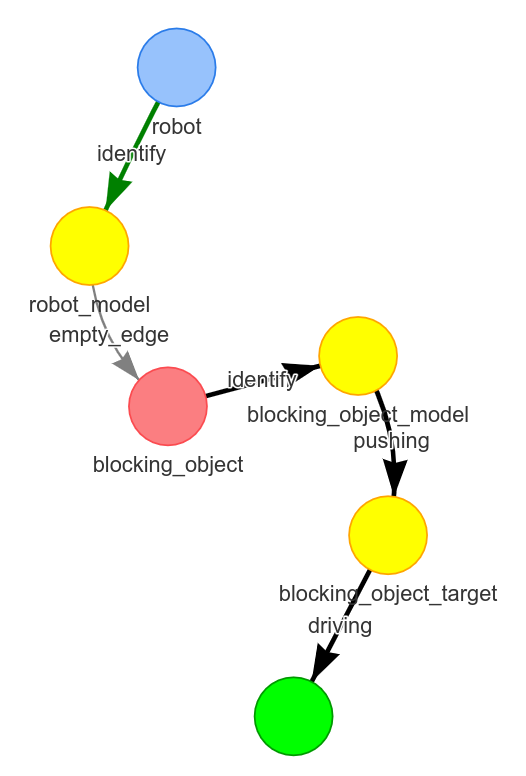
\includegraphics[width=\textwidth]{figures/proposed_method/connecting_nodes/blocking_obj/blocking_obj_3}
    \caption{}\label{subfig:blocking_obj_3}
    \end{subfigure}

    \begin{subfigure}{.3\textwidth}
    \centering
    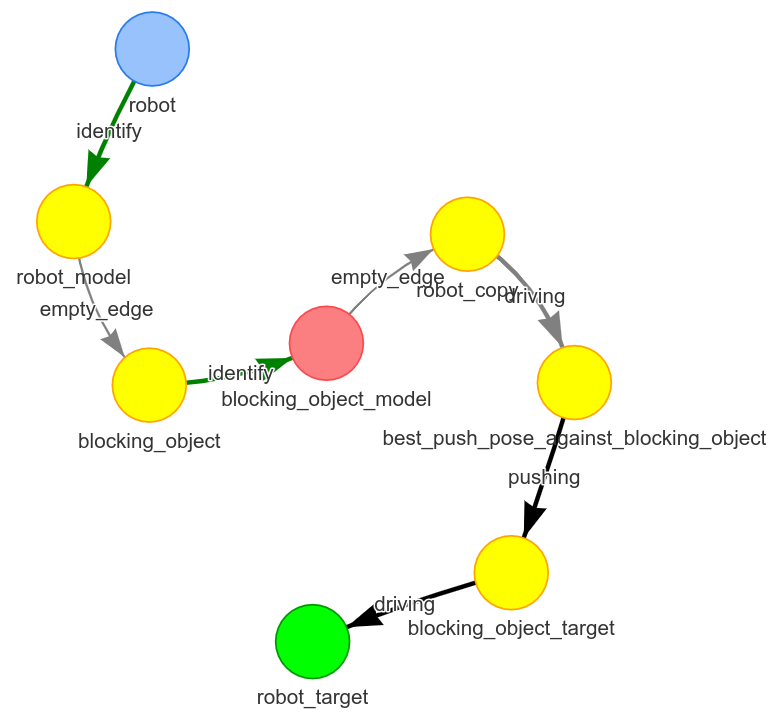
\includegraphics[width=1.291\textwidth]{figures/proposed_method/connecting_nodes/blocking_obj/blocking_obj_4}
    \caption{}\label{subfig:blocking_obj_4}
    \end{subfigure}
    \begin{subfigure}{.3\textwidth}
    \centering
    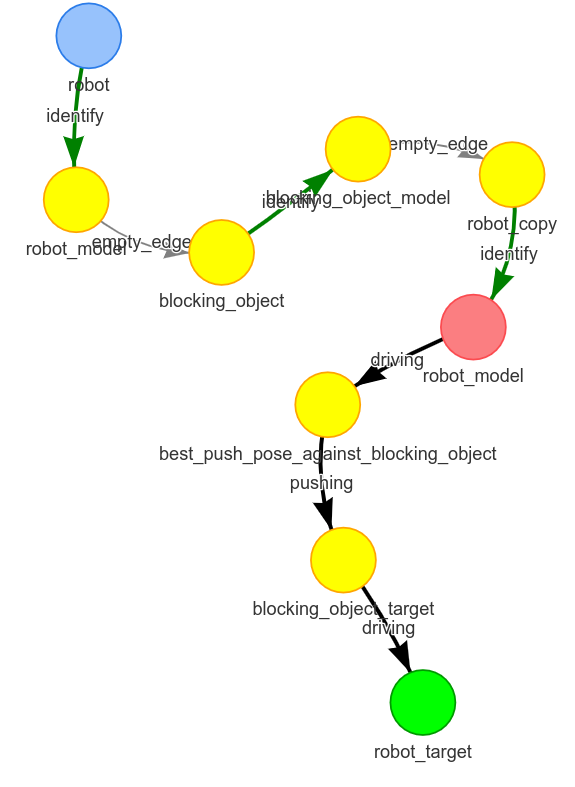
\includegraphics[width=\textwidth]{figures/proposed_method/connecting_nodes/blocking_obj/blocking_obj_5}
    \caption{}\label{subfig:blocking_obj_5}
    \end{subfigure}
    \begin{subfigure}{.3\textwidth}
    \centering
    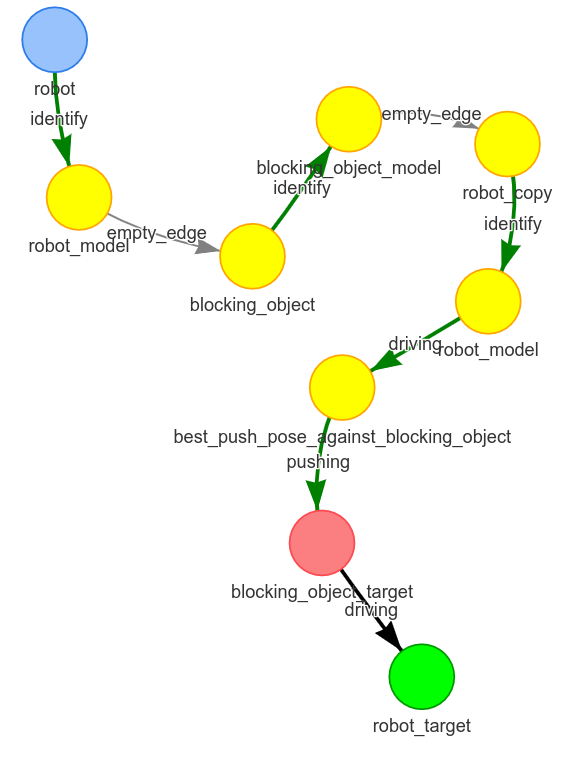
\includegraphics[width=\textwidth]{figures/proposed_method/connecting_nodes/blocking_obj/blocking_obj_6}
    \caption{}\label{subfig:blocking_obj_6}
    \end{subfigure}
    \caption{\ac{hgraph} for driving to target configuration and encountering a blocked path}%
    \label{fig:blocking_obj_hgraph}
\end{figure}

